\documentclass[a4paper,10pt]{article}

\usepackage{ucs}
\usepackage[utf8]{inputenc}
\usepackage{amsmath}
\usepackage[english]{babel}
\usepackage{fontenc}
\usepackage{graphicx}
\usepackage{tikz}
\usetikzlibrary{decorations.pathreplacing}

\usepackage{hyperref}

\date{11/22/26}

\begin{document}

\section{Optimal Stopping}

\subsection{The secretary problem}
Suppose $n$ candidates arrive in uniformly random order. All ranks are distinct,
so each of the $n!$ arrival orders is equally likely. After each interview we
can rank the candidates seen so far. We must hire or reject the current
candidate on the spot, and each rejection is final. Our goal is to maximize
the probability of hiring the single best candidate.

Choose an observation length $o$ in advance. Reject the first $o$ candidates
and remember the best of them. Hire the first subsequent candidate who beats
that benchmark. If a hire is compulsory and nobody beats the benchmark,
hire the last candidate. In that case the overall best was in the observation
phase, so the fallback cannot change the probability of success.
For $o=0$ we hire the first candidate immediately.

\begin{center}
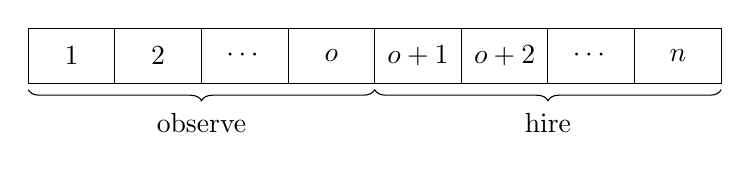
\begin{tikzpicture}[x=1.1cm]
  \draw (0,0) rectangle (8,0.7);
  \foreach \i in {1,...,7}
    \draw (\i,0) -- (\i,0.7);
  \foreach \i/\candidate in {1/1,2/2,3/\cdots,4/o,5/{o+1},6/{o+2},7/\cdots,8/n}
    \node at (\i-0.5,0.35) {$\candidate$};

  \begin{scope}[decoration={brace,mirror,amplitude=4pt}]
    \draw[decorate] (0,-0.08) -- (4,-0.08) node[midway,below=5pt] {observe};
    \draw[decorate] (4,-0.08) -- (8,-0.08) node[midway,below=5pt] {hire};
  \end{scope}
\end{tikzpicture}
\end{center}

\subsubsection*{When does the rule succeed?}
Let $B$ denote the event that we hire the best candidate, and let $h$ be that
candidate's position. For now assume $1\le o<n$. If $h\le o$, we reject the
best candidate during observation. If $h>o$, the best candidate will beat
the benchmark, but we must still be interviewing when that candidate arrives.

It is tempting to require the overall second-best candidate to appear during
observation. That would indeed set a benchmark that only the overall best
could beat. But consider arrival ranks $3,4,1,2$, where rank $1$ is best.
With $o=2$ the benchmark is rank $3$. We hire rank $1$ at the third interview,
and the runner-up arrives fourth. What matters is who appears \emph{before}
the overall best.

Suppose, for example, that we observe three candidates and the best candidate
arrives fifth. In this case $o=3$ and $h=5$. To decide whether we hire the
fifth candidate, we only need to look at the four interviews before theirs.

Now consider any position after observation and call it $k$, so $k>o$.
For the moment, suppose the best candidate arrives in that position. We write
this assumption as $h=k$. We will later add up the contributions from all
possible positions $k=o+1,\ldots,n$. Imagine drawing a line just before position
$k$. Among the $k-1$ candidates to the left of the line, let $m$ be the
position of the strongest. There are two possibilities.
\begin{itemize}
\item If $m\le o$, the strongest candidate to the left of the line set the
benchmark. Every candidate from $o+1$ through $k-1$ falls short of it.
We reach position $k$ and hire the overall best.
\item If $o<m<k$, the candidate at $m$ beats everyone in the observation
phase. We therefore hire someone by position $m$, possibly even earlier.
The interview process ends before position $k$.
\end{itemize}
Thus, given $h=k$, success is exactly the event $m\le o$.

\subsubsection*{How likely is success for a fixed cutoff?}
Conditioning on $h=k$ means imagining only orders in which the overall best
is at position $k$. Within these orders we may permute the first $k-1$
candidates freely. By symmetry their strongest member is equally likely to
occupy each of those $k-1$ positions. Exactly $o$ positions are in the
observation phase. Therefore
\[
  \Pr(B\mid h=k)=\frac{o}{k-1}\qquad(o<k\le n).
\]
For example, if $k=o+1$, the fraction is $o/o=1$. The overall best then
arrives immediately after observation, with no intervening interview at
which we could stop too early.

The letter $h$ stands for the unknown position. The letter $k$ is a running
index that takes each possible value of $h$ in turn. Each position has
probability $1/n$ of containing the best candidate. The events $h=k$ are
mutually exclusive and cover every arrival order, so the law of total
probability gives
\begin{align*}
  P_B(o)=\Pr(B)
    &=\sum_{k=1}^{n}\Pr(h=k)\Pr(B\mid h=k)\\
    &=\sum_{k=o+1}^{n}\frac1n\frac{o}{k-1}
     =\boxed{\frac{o}{n}\sum_{j=o}^{n-1}\frac1j}.
\end{align*}
The first $o$ terms vanish because we reject those candidates. In the final
sum we set $j=k-1$, so the first denominator is $o$ and the last is $n-1$.
The multiplication inside the sum uses a conditional probability. Multiplying
the marginal probabilities for the locations of the best and second-best
would also overlook their dependence: once one position is occupied, the
other candidate must occupy a different position.

\subsubsection*{Which integer cutoff maximizes this probability?}
Increasing $o$ gives a stronger benchmark on average, but costs one more
opportunity to hire. To measure the tradeoff exactly, compare $o$ with $o+1$.
For $1\le o\le n-2$, split the first term off the sum for $P_B(o)$. Then
\begin{align*}
 n\bigl(P_B(o+1)-P_B(o)\bigr)
 &= (o+1)\sum_{j=o+1}^{n-1}\frac1j
    -o\left(\frac1o+\sum_{j=o+1}^{n-1}\frac1j\right)\\
 &=\sum_{j=o+1}^{n-1}\frac1j-1.
\end{align*}
Thus one more observation helps exactly when the remaining sum exceeds $1$.
As $o$ increases, the sum decreases because we remove a positive term.
Once an extra observation hurts, every subsequent increase hurts as well.
For $n\ge2$ an optimal positive cutoff is therefore the smallest
$o\in\{1,\ldots,n-1\}$ satisfying
\[
   \boxed{\displaystyle\sum_{j=o+1}^{n-1}\frac1j\le1}.
\]
At $o=n-1$ the sum is empty and equals zero, so the rule always gives an
answer. Equality means that $o$ and $o+1$ tie. To include the option of
immediate hiring, observe that $P_B(0)=1/n$, whereas
$P_B(1)=(1+1/2+\cdots+1/(n-1))/n$. For $n>2$, observing one already beats
immediate hiring. For $n=2$ both choices tie, and for $n=1$ we hire immediately.

For example, take $n=5$. At $o=1$ the remaining sum is
$1/2+1/3+1/4=13/12>1$, so a second observation helps. At $o=2$ the
remaining sum is $1/3+1/4=7/12<1$, so a third observation hurts.
The optimal cutoff is two. If the best arrives third, fourth, or fifth,
the conditional probabilities of success are respectively $1$, $2/3$, and
$2/4$. Each position has probability $1/5$, giving
$P_B(2)=(1+2/3+2/4)/5=13/30$.

\subsubsection*{Where does the familiar 37 percent come from?}
For an exact finite-$n$ answer use the sum above. To see its large-$n$
behavior, consider observing a fraction $x$ of the candidates, where
$0<x<1$ and $o=\lfloor nx\rfloor$. Then $o/n\to x$. The sum in the success
probability becomes a Riemann sum with spacing $1/n$:
\[
  \sum_{j=o}^{n-1}\frac1j
   =\frac1n\sum_{j=o}^{n-1}\frac1{j/n}
   \longrightarrow \int_x^1\frac{dt}{t}=\log(1/x).
\]
\emergencystretch=2em
The limiting success probability is $f(x)=x\log(1/x)$. Its derivative
$f'(x)=\log(1/x)-1$ vanishes at $x=1/e$, and $f''(x)=-1/x<0$ confirms a
maximum. The exact rule gives the same limit. For any fixed fraction below $1/e$
the remaining sum tends to a value above $1$, and for any fixed fraction
above $1/e$ it tends to a value below $1$. Its crossing therefore approaches
$1/e$ as a fraction of $n$.

Hence for large $n$ we observe about $n/e$ candidates and then hire the
first who beats the observation benchmark. The fraction observed approaches
$1/e\approx0.368$. The probability of winning also approaches $1/e$,
since $f(1/e)=(1/e)\log e=1/e$.
\end{document}
